\chapter{Methodology}
\index{Methodology@\emph{Methodology}}%
\label{chap:methodology}

\section{Overview}\label{sec:method overview}




\section{ErLam}\label{sec:erlam}

\subsection{The ErLam Language}\label{sec:the erlam language}
\subsection{Channel Implementation}\label{sec:channel implementation}
\subsection{The Scheduler API}\label{sec:the scheduler api}
\subsection{Example: The CML Scheduler}\label{sec:example the cml scheduler}


\section{Simulation \& Visualization}\label{sec:simulation and visualization}

\subsection{Runtime Log Reports}\label{sec:runtime log reports}
\subsection{Cooperativity Testing}\label{sec:cooperativity testing}

As part of the thought experiment, we needed to implement a set of test cases 
which would give a decent coverage of applications which 

\begin{figure}
\centering
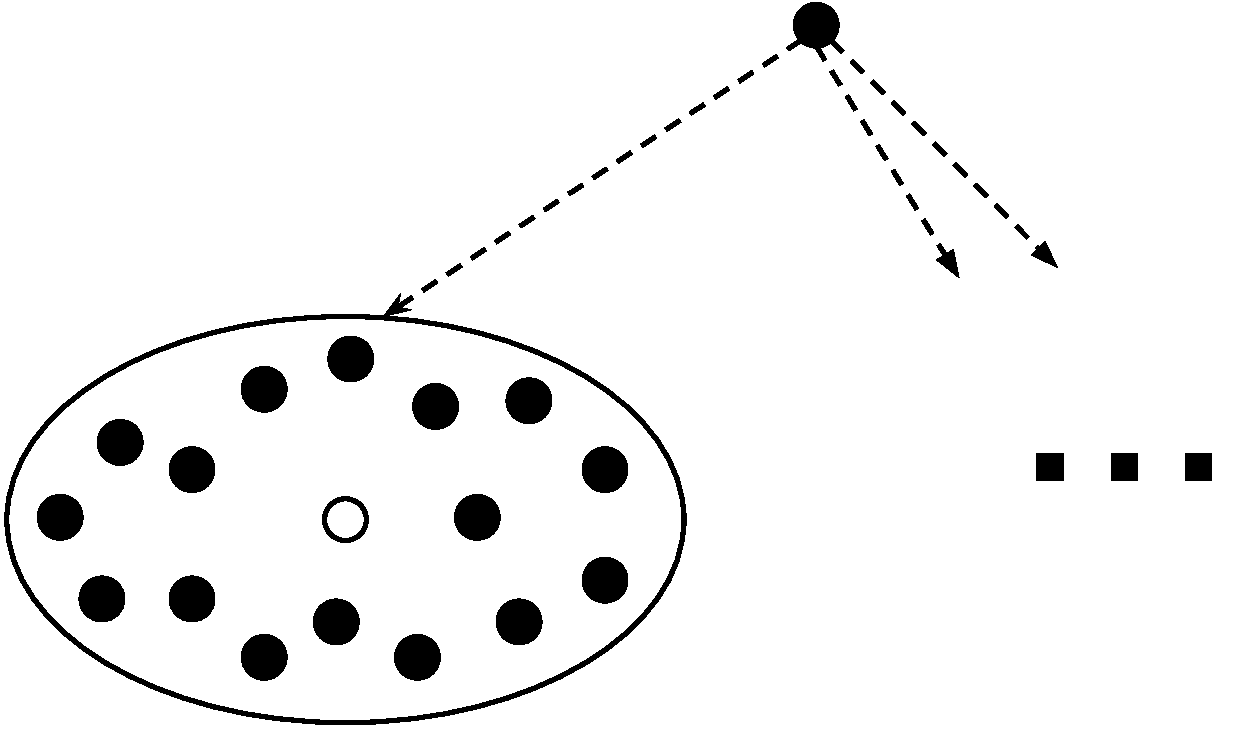
\includegraphics[scale=0.35]{PTree.pdf}
\caption{Graphical representation of $PTree$, $N$ Parallel work groups.}
\label{fig:PTree}
\end{figure}

\begin{figure}
\centering
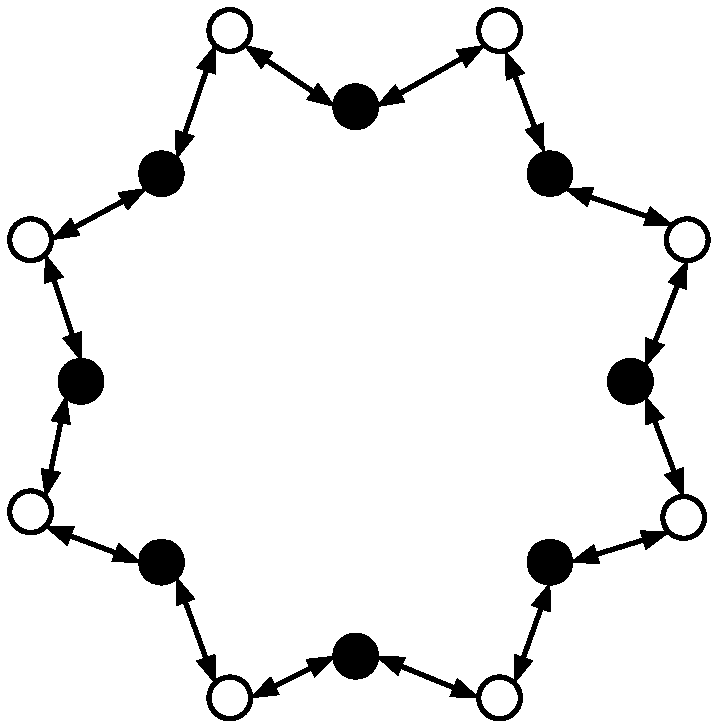
\includegraphics[scale=0.35]{PRing.pdf}
\caption{Graphical representation of $PRing$, full system predictable 
cooperation.}
\label{fig:PRing}
\end{figure}

\begin{figure}
\centering
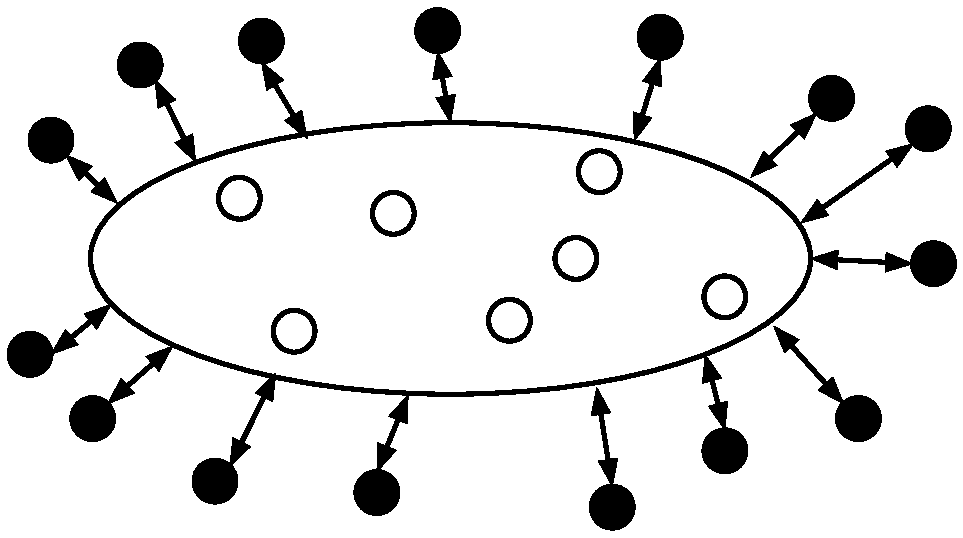
\includegraphics[scale=0.35]{ClusterComm.pdf}
\caption{Graphical representation of $ClusterComm$, $N$ processes to $M$ 
channels for unpredictable full system cooperation.}
\label{fig:ClusterComm}
\end{figure}

\begin{figure}
\centering
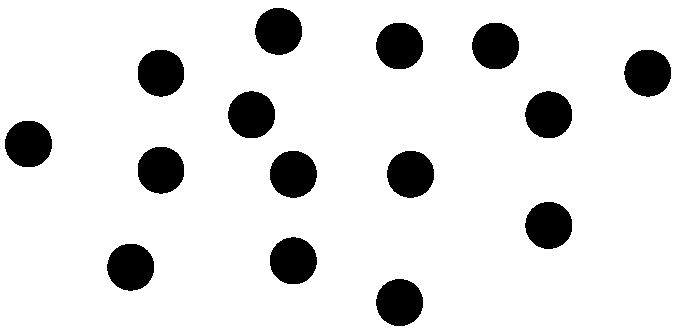
\includegraphics[scale=0.35]{ChugMachine.pdf}
\caption{Graphical representation of $ChugMachine$, $N$ worker processes 
without cooperation.}
\label{fig:}
\end{figure}

\begin{figure}
\centering
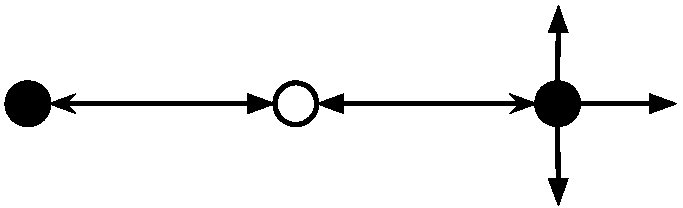
\includegraphics[scale=0.35]{UserInput.pdf}
\caption{Graphical representation of $UserInput$, single randomly hanging 
process.}
\label{fig:}
\end{figure}

\begin{figure}
\centering
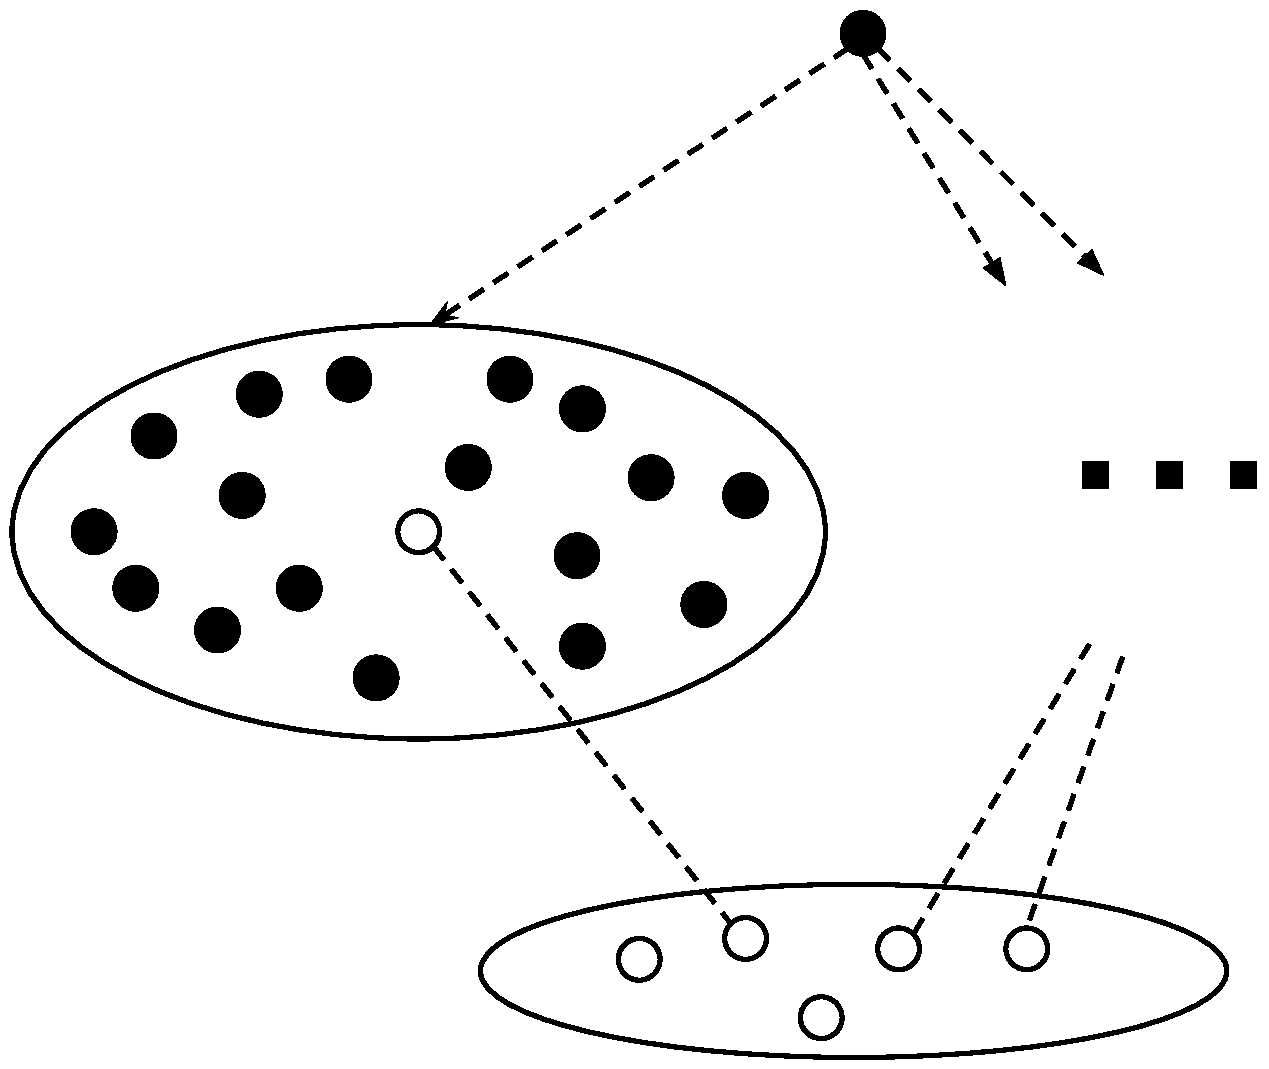
\includegraphics[scale=0.35]{JumpShip.pdf}
\caption{Graphical representation of $JumpShip$, $N$ Parallel phase shifting 
work groups.}
\label{fig:JumpShip}
\end{figure}





\section{Cooperativity Mechanics}\label{sec:cooperativity mechanics}

\subsection{Overview}\label{sec:cooperativity mechanics overview}
\subsection{Longevity-Based Batching}\label{sec:longevity based batching}
\subsection{Channel Pinning}\label{sec:channel pinning}
\subsection{Bipartite Graph Aided Shuffling}
    \label{sec:bipartite graph aided shuffling}


